\documentclass[answers]{exam}

%% Language and font encodings
\usepackage[english]{babel}
\usepackage[utf8x]{inputenc}
\usepackage[T1]{fontenc}
% \usepackage{enumitem}
%% Sets page size and margins
\usepackage[a4paper,margin=2cm]{geometry}

%% Useful packages
\usepackage{amsmath}
\usepackage{amssymb}
\usepackage{graphicx}
\usepackage{paralist}
\usepackage{framed}
\usepackage{tikz}
\usepackage{float}
\usepackage{listings}
\usepackage{xcolor}
\tikzset{
  % define the bar graph element
  bar/.pic={
    \fill (-.1,0) rectangle (.1,#1) (0,#1) node[above,scale=1/2]{$#1$};
  }
}
\definecolor{codegreen}{rgb}{0,0.6,0}
\definecolor{codegray}{rgb}{0.5,0.5,0.5}
\definecolor{codepurple}{rgb}{0.58,0,0.82}
\definecolor{backcolour}{rgb}{0.95,0.95,0.92}
% Colored Python listing from https://www.overleaf.com/learn/latex/Code_listing
\definecolor{codegreen}{rgb}{0,0.6,0}
\definecolor{codegray}{rgb}{0.5,0.5,0.5}
\definecolor{codepurple}{rgb}{0.58,0,0.82}
\definecolor{backcolour}{rgb}{0.95,0.95,0.92}
 
\lstdefinestyle{mystyle}{
    backgroundcolor=\color{backcolour},   
    commentstyle=\color{codegreen},
    keywordstyle=\color{magenta},
    numberstyle=\tiny\color{codegray},
    stringstyle=\color{codepurple},
    basicstyle=\ttfamily\footnotesize,
    breakatwhitespace=false,         
    breaklines=true,                 
    captionpos=b,                    
    keepspaces=true,                 
    numbers=left,                    
    numbersep=5pt,                  
    showspaces=false,                
    showstringspaces=false,
    showtabs=false,                  
    tabsize=2
}
\lstset{style=mystyle}

\usetikzlibrary{matrix}

\setlength\FrameSep{4pt}

\begin{document}
    \section*{Q4. Saying Random is not enough}

%--------------------------------  4.1  ------------------------------------
    \subsection*{4.1}
    \begin{framed}
        For 4.1, we took the approach specified in the question. We first pick two random angles $\theta_1$ and $\theta_2$. Then find their difference to find the angle lying in between $\theta_1$ and $\theta_2$. Then we use this new angle in \emph{cord length} formula. The program does this process 1000 times and stores the values in the specified list, then graphs a histogram for the length of the cords and the probability of them occuring. Following describes each function and their purpose/method for the program.
        \begin{enumerate}
            \item \emph{random\_theta()}: The function finds random $\theta_1$ and $\theta_2$. $\theta$ is chosen randomly from degrees($\phi$) and then converted to radians.
                    \begin{align*}
                        \theta_1 &= \phi_1 . \frac{\pi}{180}\\
                        \theta_2 &= \phi_2 . \frac{\pi}{180}
                    \end{align*}
            \item \emph{cord(R)}: The function takes the radius as the input and returns length of the cord between $\theta_1$ and $\theta_2$. It first calls \emph{random\_theta()}, and find the absolute value of their difference ($\theta=|\theta_1 - \theta_2|$). Then the length of the cord in calculated using the following formula for cord length,
                    $$\text{cord length}=2R.\sin(\theta/2)$$
            \item \emph{find\_cords1(R)}: The function takes radius R as input, then draw the histogram as the output. It iterates 1000 times, calls \emph{cord(R)} for each iteration and append the result in \emph{cord\_len}. The bin value is set to be 50 as it provides a good threshold for the 1000 values. Then it plots the graph using matplotlib.
        \end{enumerate}
    \end{framed}
    \lstinputlisting[firstline=5,lastline=34,language=python]{Q4.py}
    \begin{figure}[ht]
        \caption{Histogram of 4.1}
        \centering
        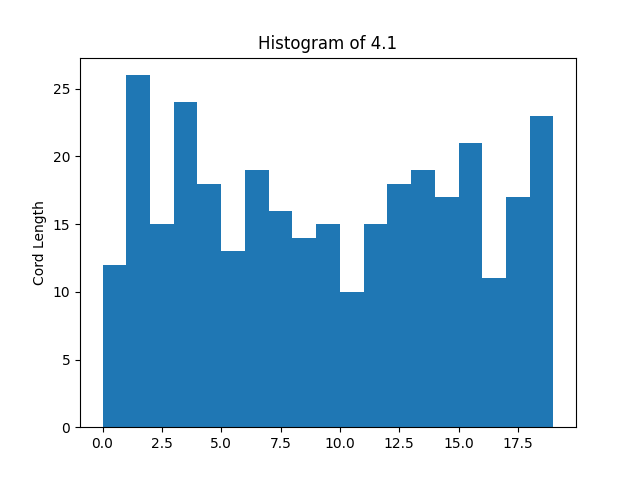
\includegraphics[scale=0.7]{Q4/Q4(1).png}
    \end{figure}
\newpage
%--------------------------------  4.2  ------------------------------------
    \subsection*{4.2}
    \begin{framed}
        For 4.2, we follow the instructions given in the question. We first pick a direction/angle and assume an imaginary radius there. Then we pick a random point on that radius and find its distance from the origin $(0,0)$. This serves as our base, while to radius R serves as our hypotaneous. Then we find the perpendicular using the pythagorean theorem, and returns the twice of it. As the perpendicular shows the half part of that cord, with randomly chosen point as its center. This point is also the midpoint for our circle, so we double the perpendicular to find the whole cord length.
        \begin{center}
            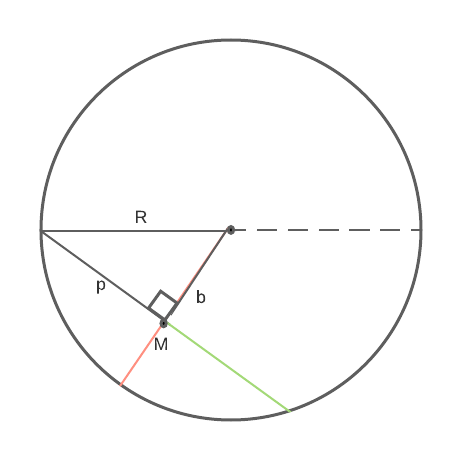
\includegraphics[scale=0.7]{Q4/4.2_circle.png}
        \end{center}
        \begin{enumerate}
            \item \emph{random\_cord(R)}: This function does multiple tasks. It first find a random direction/angle in the circle, assumes a radius on that angle, and pick a random point on the assumed radius. This point serves as the Midpoint M as well. Then it converts the polar cordinates into cartesian using the following formulae,
                \begin{align*}
                    x &= rcos(\theta)\\
                    y &= rsin(\theta)
                \end{align*}
            Then we find our base b and perpendicular p, while assuming it is a right-angle triangle because \emph{p} and \emph{b} makes a right-angle triangle. In our case we assume the distance between the origin and the random point $(x,y)$ to be our base, and radius R as our hypotaneous. We use the \emph{distance formula} to find the value of base,\\
                \begin{align*}
                    base &= \sqrt{x^2+y^2}
                \end{align*}
            Then we find the value of perpendicular line by using the pythagorean theroem,\\
                \begin{align*}
                    perpendicular &= \sqrt{R^2-base^2}
                \end{align*}
            Then we simply multiply the value of perpendicular to find the length of the cord and return it.
            \item \emph{find\_cords2(R)}: This function runs 1000 iterations of the \emph{random\_cord(R)} function, and stores their result in the list \emph{cord\_len}, sets the bin width as 50, and then graphs the histogram as the result.
        \end{enumerate}
        We run this program with radius 30. The resulting histogram seems to be an exponentially rising graph, with a flat start.
    \end{framed}
    \lstinputlisting[firstline=35,lastline=73,language=python]{Q4.py}
    \begin{figure}[h]
        \caption{Histogram of 4.2}
        \centering
        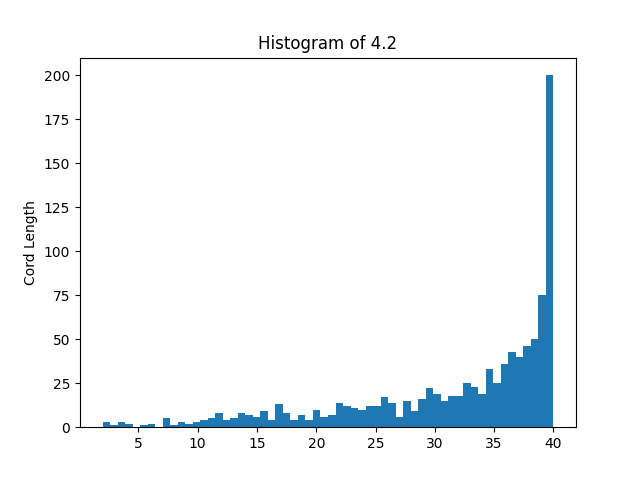
\includegraphics[scale=0.7]{Q4/Q4(2).png}
    \end{figure}
\newpage
%--------------------------------  4.3  ------------------------------------
    \subsection*{4.3}
    \begin{framed}
        For 4.3, it is similar to 4.2 with a slight difference. Instead of determining a direction, we pick a random point in the circle, and then calculates its distance from the origin $(0,0)$. If the distance is within the circle as well, we regard it as our base/adjacent of the right triangle. Then we move towards calculating the opposite/perpendicular by using pythagorean theorem, multiply it by 2 to find the total length, and then store it in the list. Then we pass that list plotting functions to plot a histogram.
        \begin{enumerate}
            \item \emph{p\_to\_o(cord)}: This function simply returns the distance between the randomly chosen point and the origin $(0,0)$. It takes a tuple of cartesian cordinates as the input and returns the distance. It uses the distance formula,
                \begin{align*}
                    dist=\sqrt{x^2+y^2}
                \end{align*}
            \item \emph{random\_point(R)}: It chooses random points for cartesian cordinates $(x,y)$ between the R and -R.
            \item \emph{cal\_cord(R,pnt)}: It takes the randomly chosen point, and finds its distance from the origin, then uses it as the adjacent/base of our right-angle triangle within the circle. Then it finds the value of the opposite/perpendicular via pythagorean theorem, and returns the twice of the opposite as the cord length.
            \item \emph{find\_cords3(R)}: This function runs 1000 times while calling the \emph{random\_point(R)} function, then it checks if the distance/base lies within the circle or not. If it does, then it proceeds to find \emph{cal\_cord(R,pnt)} and store it, else it decrements the counter by 1, to discard that value and find another.
        \end{enumerate}
        We run this program for radius 20. The histogram looks quite linear.
    \end{framed}
    \lstinputlisting[firstline=74,lastline=119,language=python]{Q4.py}
    \begin{figure}[h]
        \caption{Histogram of 4.3}
        \centering
        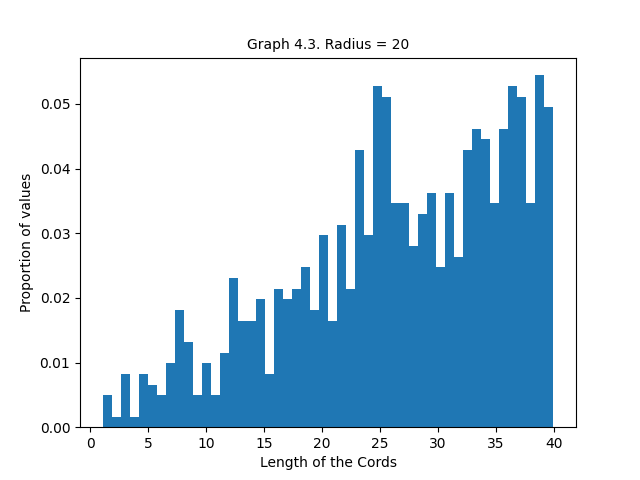
\includegraphics[scale=0.7]{Q4/Q4(3).png}
    \end{figure}
\newpage
%--------------------------------  4.3  ------------------------------------
\subsection*{4.4}
    \begin{framed}
        Out of all the distributions, I think the third approach (part 4.3) is the best to take. Its graph seems somewhat linear, which will ensure a little uniformity. As the previous graphs showed dense distribution towards the center of the circle, i.e. near the diameter, however in 4.3, the graph seems more distributed.
    \end{framed}
\end{document}